\documentclass[12pt,a4paper,notitlepage]{report}
\usepackage[utf8]{inputenc}
\usepackage[OT4]{polski}
\usepackage[T1]{fontenc}
\usepackage[top=2cm, bottom=2cm, left=3cm, right=3cm]{geometry}
\usepackage[dvipsnames]{xcolor}
\definecolor{Red}{RGB}{255,36,0}
\usepackage{changepage}
\usepackage{indentfirst}
\usepackage{color}
\usepackage{graphicx}
\definecolor{bluekeywords}{rgb}{0.13,0.13,1}
\definecolor{greencomments}{rgb}{0,0.5,0}
\definecolor{redstrings}{rgb}{0.9,0,0}
\usepackage{listings}
\lstset{language=[Sharp]C,
  showspaces=false,
  showtabs=false,
  breaklines=true,
  showstringspaces=false,
  breakatwhitespace=true,
  escapeinside={(*@}{@*)},
  commentstyle=\color{greencomments},
  keywordstyle=\color{bluekeywords},
  stringstyle=\color{redstrings},
  basicstyle=\ttfamily,
  extendedchars=true
}
\makeatletter
\newcommand{\linia}{\rule{\linewidth}{0.4mm}}
\renewcommand{\maketitle}{\begin{titlepage}
    \vspace*{1cm}
    \begin{center}\small
    Politechnika Wrocławska\\
    Wydział Elektroniki\\
    Urządzenia Peryferyjne 
    \end{center}
    \vspace{4.5cm}
    \noindent\linia
    \begin{center}
      \LARGE \textsc{\@title}
         \end{center}
     \linia
    \vspace{0.5cm}
    \begin{flushright}
    \begin{minipage}{6cm}
    
     \vspace{3cm}
     \textit{\small Termin zajęć:}\\
     \normalsize \textsc{Wtorek TN 7:30} \par
	\vspace{0.3cm}    
    \textit{\small Autorzy:}\\
    \normalsize \textsc{\@author} \par
     \vspace{0.3cm}
        Prowadzący: \\ dr inż. Tomasz Walkowiak

    \end{minipage}
    \vspace{1cm}
     {\small }\\
       
     \end{flushright}
    \vspace*{\stretch{3}}
    \begin{center}
    \@date
    \end{center}
  \end{titlepage}%
}
\makeatother
\author{ Jakub Chmiel  235028 \\ Tomasz Cieślar 235652}
\title{GPS}
\begin{document}
\maketitle

\newpage
\tableofcontents
\newpage
\renewcommand*\thesection{\arabic{section}}
\section{Cel ćwiczenia}
\begin{itemize}
\item Zapoznać się z zestawem GPS oraz podłączyć via Bluetooth
\item Odczytać uzyskane komendy oraz podzielić je wg typów wiadomości
\item Sprawdzić ważność uzyskanych danych i przedyskutować wynik
\item Obsłużyć transmisję szeregową oraz przedstawić uzyskane dane w czytelny sposób
\item Zlokalizować na mapie świata (np. z Google Map) punkty, w których znajdowało się urządzenie, na podstawie samodzielnie uzyskanych danych lub od prowadzącego (plik tekstowy, format NMEA)

\end{itemize}

\section{Wstęp}
Global Positioning System  – system nawigacji satelitarnej, stworzony przez Departament Obrony Stanów Zjednoczonych, obejmujący swoim zasięgiem całą kulę ziemską. System składa się z trzech segmentów: segmentu kosmicznego – 31 satelitów orbitujących wokół Ziemi na średniej orbicie okołoziemskiej; segmentu naziemnego – stacji kontrolnych i monitorujących na Ziemi oraz segmentu użytkownika – odbiorników sygnału. Zadaniem systemu jest dostarczenie użytkownikowi informacji o~jego położeniu oraz ułatwienie nawigacji po terenie.

NMEA – opublikowany przez National Marine Electronics Association protokół komunikacji między morskimi urządzeniami elektronicznymi. Ma on powszechne zastosowanie w elektronice nawigacji morskiej oraz urządzeniach GPS.

Dane są transmitowane w postaci „zdań” zapisanych kodem ASCII. Pojedyncza sekwencja zawiera do 82 znaków. Znakiem zaczynającym dane w protokole jest znak „\texttt{\$}”, dalej następuje identyfikator zdania i pola danych oddzielone przecinkami, a na końcu znajdują się symbole <CR><LF> (carriage return, line feed).

\section{Założenia projektowe}
\begin{itemize}
\item Program był pisany w języku C\texttt{\#}.
\item Na komputerze, na którym uruchamiany był program zainstalowano system operacyjny Windows 10 w wersji 64-bitowej.
\end{itemize}

\section{Wykorzystane narzędzia}
\begin{itemize}
\item 32feet.NET - NuGet umożliwiający korzystanie z technologii Bluetooth, IrDA i OBEX w platformie .NET.
\item NMEAParser GhostWare - NuGet do parsowania wiadomości NMEA w języku C\texttt{\#}
\item Windows Forms - API do implementacji interfejsu graficznego dla platformy .NET.\end{itemize}
\begin{adjustwidth}{0pt}{-50pt}
\section{Implementacja programu}
\subsection{Interfejs użytkownika}
\noindent 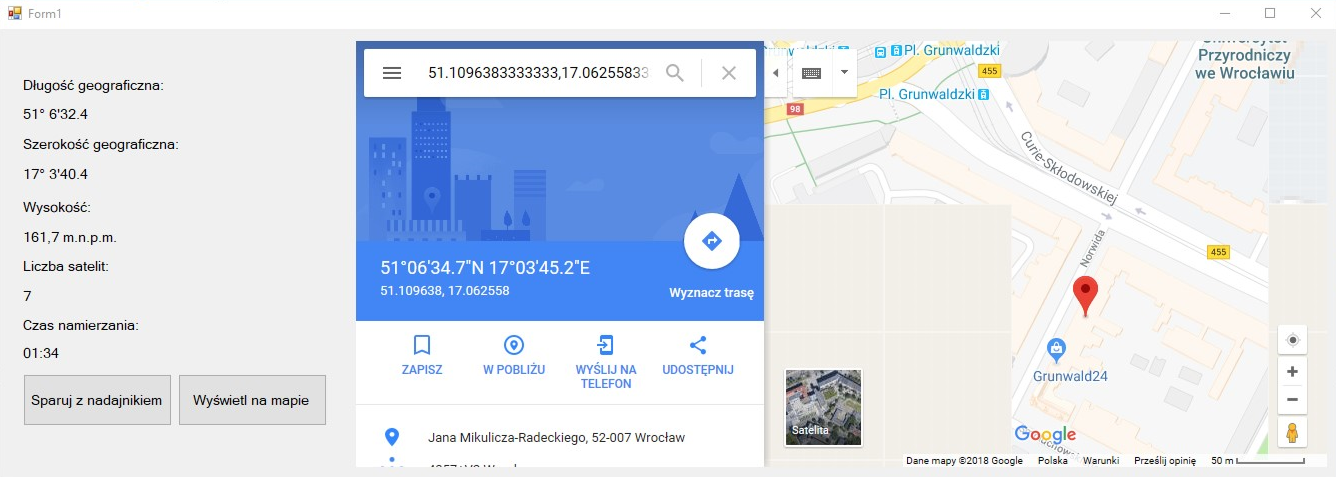
\includegraphics[scale=0.45]{okno}
\begin{center}
\footnotesize \textit{Rysunek 1. Interfejs aplikacji}
\end{center}
\subsection{Kod programu}
\begin{lstlisting}
using [...]
namespace WindowsFormsApp2
{
    public partial class Form1 : Form
    {
        private string _latitudeFinal;
        private string _longtitudeFinal;
        private string _satellitesNumberFinal;
        private string _altitudeFinal;
        private string _longMap;
        private string _latMap;
        private Stopwatch _stopwatch;
        private Timer _timer;
        static readonly BluetoothClient BluetoothClient = new BluetoothClient();

        public Form1()
        {
            InitializeComponent();
            latValue.Text = "";
            longValue.Text = "";
            altValue.Text = "";
            satNumValue.Text = "";
            timerLabel.Text = "";
        }
        
        public void Pair()
        {
            //Wyszukanie wszystkich urzadzen BT
            var allBtDevices = BluetoothClient.DiscoverDevices();
   
            //Zabranie urzadzenia o pozadanej nazwie (nadajnik Pentagram)
            var wantedDevice = allBtDevices.Where(x => x.DeviceName.Equals("PENTA-GPS")). FirstOrDefault();
            if (wantedDevice != null)
            {
                //Parowanie urzadzenia
                wantedDevice.Update();
                wantedDevice.Refresh();
                if (BluetoothSecurity.PairRequest(wantedDevice. DeviceAddress, "0000"))
                {
                    MessageBox.Show("Urzadzenie sparowane pomyslnie");
                    //Asynchroniczne polaczenie z urzadzeniem. Po pomyslnym wykonaniu polaczenia przechodzimy do metody Connect
                    BluetoothClient.BeginConnect(wantedDevice. DeviceAddress, BluetoothService.SerialPort, new AsyncCallback(Connect), wantedDevice);
                    _timer = new Timer { Interval = (1000) };
                    _timer.Elapsed += new ElapsedEventHandler(TimerTick);
                    _stopwatch = new Stopwatch();
                    _timer.Enabled = true;
                    _timer.Start();
                    _stopwatch.Start();
                }
                else
                {
                    MessageBox.Show("Nie udalo sie sparowac urzadzenia.");
                }
            }
        }

        private void Connect(IAsyncResult result)
        {
            

            if (result.IsCompleted)
            {
                //Pobieramy strumien danych z urzadzenia
                var nsFromDevice = BluetoothClient.GetStream();
                while (true)
                {
                    if (nsFromDevice.CanRead)
                    {
                        //Bufor dla odebranej wiadomosci
                        var bufferMessage = new byte[256];
                        var completeMessage = new StringBuilder();
                        
                        do
                        {
                            var numberOfBytesRead = nsFromDevice.Read(bufferMessage, 0, bufferMessage.Length);

                            completeMessage.AppendFormat("{0}", Encoding.ASCII.GetString (bufferMessage, 0, numberOfBytesRead));
                        }
                        while (nsFromDevice.DataAvailable);
                        try
                        {
                            //Parsowanie wiadomosci w formacie NMEA
                            var nmeaParser = new NmeaParser();
                            var parsedMessage = (GpggaMessage)nmeaParser.Parse (completeMessage.ToString());
                            Console.WriteLine("Odebrano nastepujaca wiadomosc: " +
                                 completeMessage.ToString());
                            this.ShowParsedMessage (parsedMessage);
                        }
                        catch (Exception exc)
                        {
                            Console.WriteLine("Wystapil blad, ponowna proba pobrania danych");
                            Console.WriteLine();
                        }
                    }
                    else
                    {
                        Console.WriteLine("Nie mozna odczytac danych z tego strumienia.");
                    }
                }
            }
        }

        public void ShowParsedMessage(GpggaMessage parsedMessage)
        {
            //Szerokosc geograficzna

            //Poszczegolne skladowe wspolrzednych geograficznych
            var minutes = (parsedMessage.Latitude - Math.Floor(parsedMessage.Latitude)) * 60.0;
            var seconds = (minutes - Math.Floor(minutes)) * 60.0;
            var tenths = (seconds - Math.Floor(seconds)) * 10.0;

            //Formatowanie szerokosci na potrzeby wyswietlenie polozenia na mapie
            _latMap = parsedMessage.Latitude.ToString();
            _latMap = _latMap.Replace(',', '.');

            //Usuniecie ulamkow
            minutes = Math.Floor(minutes);
            seconds = Math.Floor(seconds);
            tenths = Math.Floor(tenths);
            _latitudeFinal = Math.Floor(parsedMessage.Latitude) + " " + minutes + "'" + seconds + "." + tenths;

            //Analogicznie dla dlugosci geograficznej

            minutes = (parsedMessage.Longitude - Math.Floor(parsedMessage.Longitude)) * 60.0;
            seconds = (minutes - Math.Floor(minutes)) * 60.0;
            tenths = (seconds - Math.Floor(seconds)) * 10.0;

            _longMap = parsedMessage.Longitude.ToString();
            _longMap = _longMap.Replace(',', '.');

            minutes = Math.Floor(minutes);
            seconds = Math.Floor(seconds);
            tenths = Math.Floor(tenths);

            _longtitudeFinal = Math.Floor(parsedMessage.Longitude) + " " + minutes + "'" + seconds + "." + tenths;

            //Wysokosc n.p.m.
            _altitudeFinal = parsedMessage.Altitude + " m.n.p.m.";

            //Liczba satelit
            _satellitesNumberFinal = parsedMessage.NumberOfSatellites.ToString();
        }

        private void btShowMap_Click(object sender, EventArgs e)
        {
            //Przejscie do Google Maps na znalezionym punkcie
            wbMap.Navigate("https://www.google.com/maps/?q=" + _latMap + "," + _longMap);
        }

        private void btPair_Click(object sender, EventArgs e)
        {
            //BackgroundWorker odpowiada za aktualizacje informacji na ekranie

            var backgroundWorker = new BackgroundWorker();
            

            backgroundWorker.WorkerReportsProgress = true;

            backgroundWorker.DoWork += new DoWorkEventHandler(
                delegate (object o, DoWorkEventArgs args)
                {
                    var secondaryBw = o as BackgroundWorker;

                    for (int i = 1; i <= 1000; i++)
                    {
                        secondaryBw.ReportProgress(i * 10);
                        Thread.Sleep(1000);
                    }
                });
            
            backgroundWorker.ProgressChanged += new ProgressChangedEventHandler(
                delegate (object o, ProgressChangedEventArgs args)
                {
                    latValue.Text = _latitudeFinal;
                    longValue.Text = _longtitudeFinal;
                    altValue.Text = _altitudeFinal;
                    satNumValue.Text = _satellitesNumberFinal;
                });

            backgroundWorker.RunWorkerCompleted += new RunWorkerCompletedEventHandler(
                delegate (object o, RunWorkerCompletedEventArgs args)
                {
                    satNumValue.Text = "Ukonczono!";
                });

            backgroundWorker.RunWorkerAsync();
            Pair();
        }
        //Odmierzanie czasu od rozpoczecia namierzania
        void TimerTick(object sender, ElapsedEventArgs e)
        {
            timerLabel.BeginInvoke(new MethodInvoker(() => timerLabel.Text = _stopwatch.Elapsed.ToString("mm\\:ss")));
        }
    }
}


\end{lstlisting}
\end{adjustwidth}
\section{Wnioski}
W ćwiczeniu wykorzystaliśmy wiedzę nabytą w trakcie zajęć z Bluetooth. Bardzo przydatny okazał się NMEAParser GhostWare, dzięki niemu mogliśmy w łatwy sposób przekształcić zakodowaną wiadomość wysyłana przez modem GPS na przyjazną w odbiorze, wyświetlaną w programie.
\section{Bibliografia}
\begin{enumerate}
\item Dokumentacja 32Feet.NET:\\$http://inthehand.github.io/html/R\_Project\_InTheHand.htm$
\item Parser wiadomości NMEA:\\$https://github.com/kevingoos/NMEAParser$
\item GPS:\\$https://pl.wikipedia.org/wiki/Global\_Positioning\_System$
\item NMEA:\\$https://pl.wikipedia.org/wiki/NMEA\_0183$

\end{enumerate}
\end{document}